\chapter{State of the art}
\label{capitolo2}
\thispagestyle{empty}

 This chapter reports an overview of research works regarding the task of door finding performed by autonomous robots. After a small introduction, we report the most relevant doors detection approaches based on handcrafted features extracted from visual data. Due to the predominant role that deep learning methods have acquired in Computer Vision tasks (like image classification and segmentation, scene understanding, and object detection), we survey the evolution of end-to-end methods to perform object detection. Then, we present relevant approaches to detect doors by mobile robots that exploit the advantages of deep models. The next section of this chapter surveys the open problems and challenges of Deep Learning applied to robotic vision applications. Finally, we define the importance of simulations to acquire well-formed datasets for training and testing end-to-end models engaged in robotics contexts.  
 
 Mobile robots are active agents that operate interacting with the real world. To successfully execute the assigned task, a mobile robot has to build an abstract model of the environment in which it operates. Considering indoor scenes, doors are crucial features that a robot can acquire to make its environment's model more informative. 
 Smart vacuum cleaners, healthcare robots or intelligent housekeepers help people in their daily tasks. Usually, the tasks assigned to these autonomous agents imply moving between rooms and dealing with doors. The capabilities to detect doors, called \emph{doors detection}, can help robots to safely navigate in indoor environments, by improving their planning abilities and navigation strategies \cite{sonarandivisualdoordetection, doorsandnavigation, humanoid}.
 
 \section{Doors Detection using Handcrafted Features}
  In literature, there are a lot of different studies concerning doors detection. One of the firsts attempts, described in \cite{sonarandivisualdoordetection}, combines visual information and sonar sensors to safely traverse doors by a B21 robot. Doors present a challenging obstacle for this agent, so the goal consists of traversing opened doors using a certain angle to avoid collisions. This activity is divided into two sub-tasks: door detection and door crossing. The first one is of interest to this thesis. \citeauthor{sonarandivisualdoordetection}, \cite{sonarandivisualdoordetection}, consider an opened door as a squared noisy rectangular segment in an image. To detect it, this approach applies a vertical Sobel Filter to the grayscaled image. If it is detected a column wider than a certain threshold, it is considered a door. The sonar sensors are used to obtain the robot's distance from possible doors, to confirm the matches and avoid false positives (wrong recognition of doors).
  
  The method of \cite{humanoid} proposes a solution to detect both a door and its knob by a humanoid robot. This solution recognizes the door's features and works sufficiently fast to perform online. \citeauthor{humanoid} \cite{humanoid} argue that a door does not have very discriminative features, and the door's appearance can vary dramatically as viewpoint changes. To solve this issue, the proposed method at first extracts features points from input frames using an optimized version of the CenSurE filter, described in \cite{censure}.  Then, the Randomized Tree algorithm classifies these features to determine if a frame contains a door (the approach is reported in \cite{treefeature}). The tree predictor is trained offline using the feature points extracted from \emph{base images} previously acquired in the real environment. If a door is detected, the robot walks toward the door and localizes its knob using a segmentation technique and some general constraints (size, ratio, and height bounds).
  
  Another method for recognizing doors in unfamiliar environments is described in \cite{edgeandcornerdoorsdetector}. In this work, doors are considered significant landmarks for navigation and self-localization not only for an autonomous agent but also for blind people. This method takes into account of a variety of conditions, including differences in illumination, scale changes, deformation caused by perspective and occlusion, and variance of doors’ color, texture, or appearance.  
   At first, images are converted in grayscale and smoothed by Gaussian lowpass filter. Then, edges and corners are extracted from the pre-processed frames, using respectively the Canny Edge Detector, \cite{canny}, and the method described in \cite{cornerdetector}. The authors then define a geometric shape model of doors, which is composed of two horizontal and two vertical lines between four corners. These features are then aggregated to find possible doors: only those groups that match the model are considered as true positives.  
   
   \begin{figure}[h!]
   	\centering
   	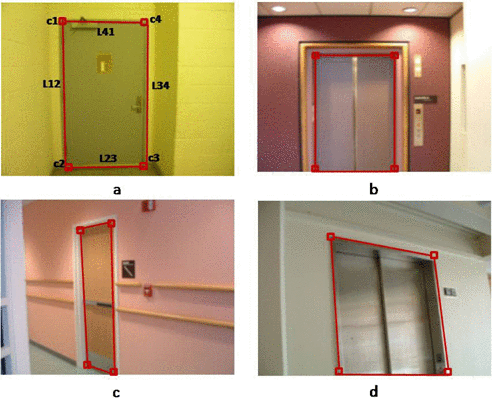
\includegraphics[width=0.65\linewidth]{images/corner_door.png}
   	\caption{The geometric model of a door (a). The ideal model (b).   The model with occlusion (c) and perspective deformation (d). Image from \cite{cornerdetector}.}
   \end{figure}
 
 \section{Deep Learning in Object Detection}
 As the performance of hand-crafted features based detectors are unable to increase, Computer Vision researchers started to use Deep Learning methods for object detection. Today object detection strongly depends on the power of Deep Learning. \citeauthor{computervisionsurvey} in \cite{computervisionsurvey} survey the history of the most relevant approaches to perform this challenging task. 
 
 After the reborn of Convolutional Neural Networks (CNNs) in 2012, \citeauthor{rcnn} propose in \cite{rcnn} the first Deep Learning paradigm to detect objects, called RCNN (Region with CNN features). RCNNs, described in \cite{rcnn}, consists of three modules. The first generates category-independent region proposals, that are sub-portion of the same image. The second module is a large convolutional neural network (CNN) that extracts a fixed-length feature
 vector from each region. The third module is a set of class-specific linear SVMs, that predict the presence of an object within each region proposal using the relative feature vectors. Despite the great progress brought by RCNN, its drawback is obvious: the detection speed is extremely slow (about 14s per
 image with GPU). This is caused by the redundant feature computation over a large number of overlapped region proposals (over 2000 per image).
 
 To overcome this limitation, \citeauthor{sppnet} propose in \cite{sppnet} the Spatial Pyramid Pooling Networks (SPPNets). This new network computes a single feature map of the entire image and then associates these features to the correspondent region proposal. This method avoids the repeatedly feature extraction phase from overlapped sub-portions of the same image.  Unlike the classic CNNs, SPPNet accepts as input images of arbitrary size and generates a fixed-length representation regardless of image size/scale. 
 
 In \cite{fastrcnn}, \citeauthor{fastrcnn} describes a new detector called Fast RCNN. This work unifies in the single end-to-end module the CNN responsible to extract features and the bounding box regressor, improving training and testing speed while also increasing accuracy. 
 
 The next step is to generate object proposals directly with a CNN model. This technique is explained in \cite{fasterrcnn}, where \citeauthor{fasterrcnn} introduce Faster RCNN: the first near-realtime
 end-to-end Deep detector. The main contribution of this work is the Region Proposal Network (RPN) that simultaneously predicts object bounds and objectness scores at each position. Since that RPN is a convolutional network, it can be trained jointly with the entire model by sharing convolutional layers in a unique end-to-end learning framework. The training procedure alternates between fine-tuning for the region proposal task and object detection phase keeping the proposal regions fixed. 
 
 The methods described before are also defined ``two-stage detectors'', because they frame the detection as a ``coarse-to-fine'' process. Its evolution is a new paradigm called ``one-stage detectors'', where the detection process is performed in a single step.  In \cite{yolo}, \citeauthor{yolo} present YOLO (You Only Look Once), a novel neural network that doesn't follow the first detection paradigm based on ``proposal detection + verification''. YOLO, who is applied to the full image, divides a frame into a grid and predicts bounding boxes and class probabilities for each cell simultaneously. YOLO is also the first real-time detector: its runs at 45fps while a lighter implementation reaches 155 fps (though with less detection quality).  Later, several improvements have been made to YOLO. \citeauthor{yolov2}  proposed the v2 and v3 editions \cite{yolov2, yolov3}, improving both detection speed and accuracy.
 
  \begin{figure}[h!]
 	\centering
 	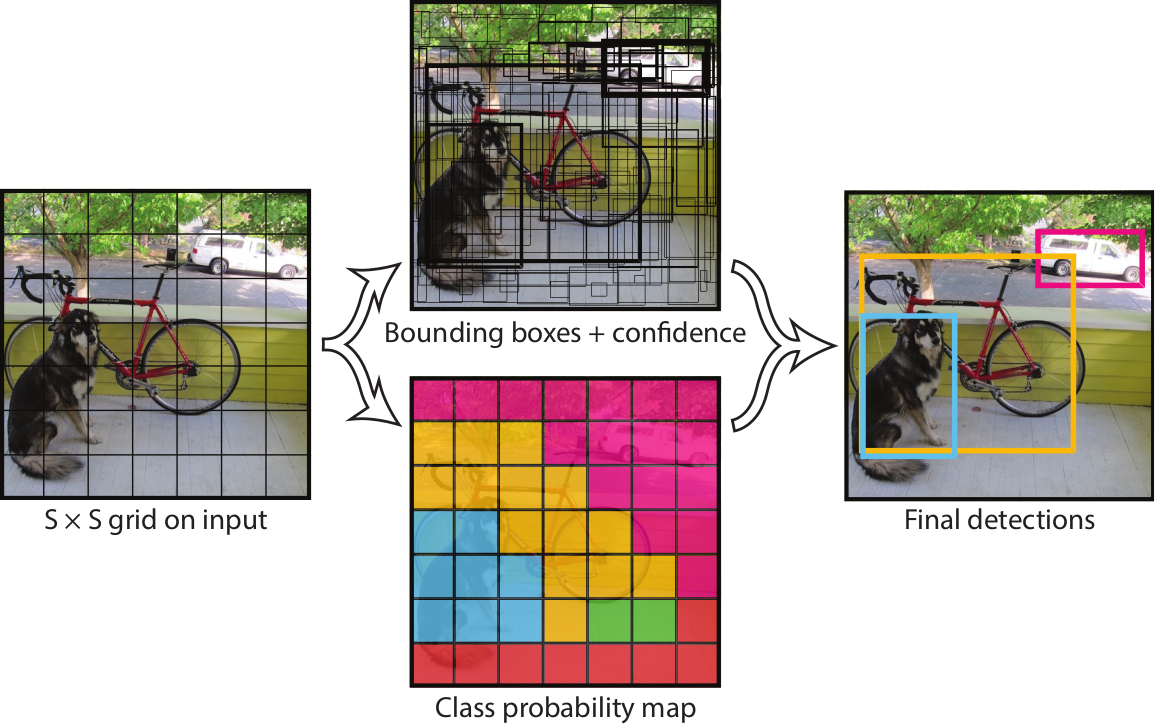
\includegraphics[width=0.8\linewidth]{images/yolo.png}
 	\caption{The detection mechanism of YOLO, the first one-stage detector. YOLO models detection as a regression problem. It divides the image into an $S \times S$ grid and for each grid cell predicts $B$ bounding boxes, confidence for those boxes,
 	and $C$ class probabilities. These predictions are encoded as an
 	$S \times S \times (B * 5 + C)$ tensor. Image from \cite{yolo}.}
 \end{figure}
 
 Despite these great results, YOLO suffers from localization accuracy compared with two-stage detectors, especially for small objects. The second one-stage detector is called SSD (Single Shot MultiBox Detector), presented in \cite{ssd}. In this work, the authors introduce the multi-reference and multi-resolution detection techniques. The main idea is to define a set of anchor boxes with different scales and aspect ratios at different locations of the same image, and then predict the bounding boxes and their class using these references. Using this method, SSD significantly improves the detection performance, also for small objects. 
 
 Despite their fast computation, one-stage detectors are not yet able to overcome two-stage detectors in accuracy. In \cite{focalloss}, \citeauthor{focalloss} discover the reason behind this fact: it consists of the extreme foreground-background class imbalance encountered during training. Following this intuition, the authors propose in \cite{focalloss} a new loss function, called Focal Loss, to put more focus on hard misclassified examples during training. Thanks to Focal Loss, the one-stage detectors achieve an accuracy comparable to that of the two-stage detectors, while maintaining very high detection speed. In their work presented in \cite{focalloss}, \citeauthor{focalloss} design a simple end-to-end module called RetinaNet to demonstrate the effectiveness of their proposed loss function. 
 
 More recently in \cite{transformer}, \citeauthor{transformer} propose a new end-to-end paradigm called Transformer, who demonstrate state-of-the-art results in Natural Language Process tasks, e.g. text classification, machine translation, and question answering. Transformers are based on encoder-decoder architectures with self-attention mechanism. In a sequence of items, the self-attention technique estimates the relevance of each item to the others, capturing the interactions between them. This enables Transformers to model long dependencies between input sequence elements and support parallel processing. 
 
 This new architecture intrigued researchers to study its application to Computer Vision problems. In \cite{surveytransformer}, \citeauthor{surveytransformer} survey the history of Transformers' implication in Computer Vision. \citeauthor{detr}, \cite{detr}, present DETR (DEtection TRansformer), the first end-to-end model based on Transformer to perform object detection. DETR extracts features from an image using a CNN backbone and then feeds them into a classic transformer to capture their relationships. Its outputs are post-processed by a linear regressor and a multilayer perceptron, that infer the category labels and the bounding boxes, respectively.
 
 \section{Doors Detection with Deep Learning} 
 Deep learning methods outperform traditional approaches in Computer Vision \cite{deeplearningoverview}. This is because classic methods based on handcrafted features are not generalizable, meaning the features (like edges or corners) needs to be specifically aggregated for different object categories. An end-to-end module, instead, learns automatically how to extract useful features that characterize an object. In particular, it extracts low-level features, corners or edges, in early stages, and then aggregates them in a more complex manner. It is well known that these features are robust to scale, shift, rotation, and exposure changes. Given their advantages, end-to-end modules have become widely used in robotics, including the task of doors detection.
 
 The method proposed in \cite{detectdoorsfeature} is a vision-based technique for detecting doors by an autonomous agent. The main idea is to consider only color and shape information as useful features to detect doors in an office. This approach uses two neural classifiers to recognize these specific components in an image. One is trained for detecting the top, left, and the right bar of the door while the other is trained for detecting the door's corners. Then, a heuristic algorithm combines these features and checks if they match a typical door structure. A door is detected if at least three of these features are found in a frame and they comply with the door's geometrical constraints. 
 
 Robot navigation, which denotes the robot's ability to establish its own position and orientation within the frame of reference, is a challenging task for autonomous systems, especially in unknown and dynamic environments. The method described in \cite{doorsandnavigation} performs doors detection to improve the navigation strategy of autonomous agents. This approach uses a convolutional neural network to detect doors in an indoor environment. For each door in the training dataset, the proposed approach collects five images taken from different locations. The final goal is to give to the robot the location of doors, then make decisions of how to move to the doors and go through them.
 
 Another approach, described in \cite{doorcabinet}, focuses on robustly identify doors, cabinets, and their respective handles for robot grasping. The authors use a Convolutional Neural Network (based on YOLO) to detect the ROI (region of interest) of doors. Then, the proposed method obtains handle's point cloud using two different approaches. The first one is a visual segmentation approach based on k-means color clusterization of the ROI while the former is a plane model extraction of the point cloud generated inside the region of interest. The ROI significantly reduces computational time and false-positive rates in the previous two phases.
 
 \section{The Limits of Deep Learning for Robotics}
 
 Despite the advantages and the excellent results of deep learning techniques, their application in robotics leads to specific problems and challenges that are not addressed by Computer Vision researchers. This is because a robot is an active agent that interacts with the real world and often operates in uncontrolled or challenging conditions. Mistakes can lead to potentially catastrophic results and can even put human lives at risk, e.g., if the robot is an autonomous vehicle. In \cite{surveydeeplimits}, \citeauthor{surveydeeplimits} investigate the challenges of Deep Learning applied to robotics. They define the concept of Robotic Vision, which highly differs from Computer Vision. While the latter translates images into information, Robotic Vision translates images into actions, performed in the real world. For an autonomous agent, perception is only a small part of a more complicated and goal-driven system. 
 
 \begin{figure}[h!]
 	\centering
 	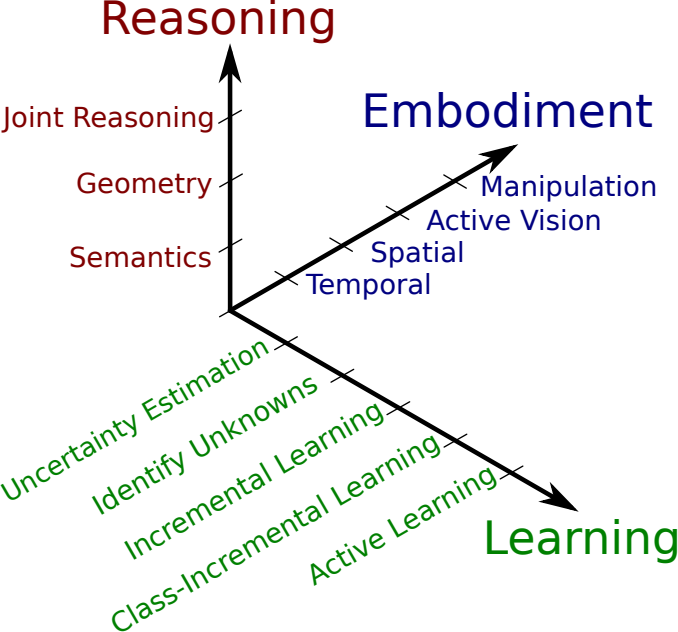
\includegraphics[width=0.6\linewidth]{images/rvchallenges.png}
 	\caption{Current Challenges for Deep Learning in Robotic Vision. The authors categorize these challenges into three conceptually orthogonal axes:
 		learning, embodiment, and reasoning. The learning axis is of interest for this thesis. Image from \cite{surveydeeplimits}.}
 \end{figure}
 
 The authors also survey the most most important learning challenges for a (deep) learning machine in a Robotic Vision context. The first is \textit{uncertainty estimation}. An autonomous agent has to estimate the uncertainty of its deep learning modules, considering them in the same way as other sensors. This is not trivial because deep entities return scores that are not calibrated probabilities, so their outputs are not usable in a Bayesian sensor fusion framework, as commonly done in robotics to improve robustness. In Deep Learning, it is assumed that a model operates in \textit{close-set} condition,  i.e., the classes encountered during deployment are known and exactly the same as during training. However, an autonomous agent operates in real-world environments that are uncontrolled and extremely different from each other. In this context, a robot will encounter instances of classes, scenarios, textures, or environmental conditions that were not covered by the training data. On this \textit{open-set} conditions, it is crucial to identify the unknowns, not recognizing them as known classes. Other important challenges for robotics applications using Deep Learning are \textit{incremental learning} and \textit{class-incremental learning}. The characteristics and appearance of objects may change a lot in the deployment scenario compared with the training phase. In addition, real environments often include new objects' categories, not included in the training data. To address this limitation, a Robotic Vision system should be able to learn from new training samples of known and unknown classes collected during deployment. Current techniques for incremental learning imply supervision, in the sense that a human operator has to select and annotate the new data to incorporate in the deep model. \textit{Active learning} is the challenge to overcome this limitation. To minimize user interaction, a robot should be able to select autonomously the best samples to increment the training data and specialize its deep models. In \cite{surveydeeplimits}, \citeauthor{surveydeeplimits} also pose attention on datasets and metrics used to train and evaluate end-to-end modules. As mentioned before, a (deep) model used by an autonomous agent operates in \textit{open-set} conditions when only a small and incomplete knowledge of the real world has been used during training. Following this intuition, the authors argue that the most known and challenging datasets used in Computer Vision (e.g. COCO \cite{coco} or Pascal VOC \cite{pascal}) are not able to model the \textit{open-set} conditions in which a Robotic Vision model operates. This is because they offer a huge amount of data related only to specific object categories, making them unable to represent unknown object classes. Also the metrics (e.g. average accuracy, area under the curve, precision, recall) are not able to measure the uncertainty. These measures compute the best summary statistic over a canned dataset, so they do not generalize well to the entire problem. These metrics indicate that a dataset has been solved, but it does not necessarily mean that the problem itself has been solved.  
 
 
 \section{The Role of Simulation for Robotics}
 \label{sec:importanceofsimulation}
 As argued by \citeauthor{surveydeeplimits} in \cite{surveydeeplimits}, there is a lack of vision datasets for robotic applications, so data collection is a crucial phase to exploit a Robotic Vision task. Modern deep learning models are extremely data hungry: they need a large amount of data to converge and the examples must be as heterogeneous as possible. Besides the size, a well-formed dataset usable in Robotic Vision applications should be able to well generalize the problem it represents. The images should be captured from different positions, heights, and illumination conditions to emulate the freedom of movement that characterizes an autonomous robot. In addition, the examples should be collected from a large numbers of scenes and building types, considering indoor environments with different designs, furniture styles, and structural features. A single object radically changes its appearance based on the context to which it belongs. To collect a dataset from the real world is extremely time expensive and costly. This is because the high number of robot runs to perform, the large amount of environment to consider, and the physical configuration of the active agent employed. To cope with these limitations, simulations are widely used for this purpose. 
 
 Gibson Environment, presented in \cite{gibson}, is a real-world perception framework that can be used to acquire the necessary examples for developing robotic visual perception models. Gibson virtualizes scanned real spaces, rather than using artificially designed ones. Through Gibson, an arbitrary agent (e.g. a small robot as a Turtlebot \cite{turtlebot2, turtlebot3}, a humanoid, or a car) can be simulated respecting its physical constraints, as well as those of the real world. Gibson provides a stream of visual observations from arbitrary viewpoints as if the agent had an on-board camera. The observations include RGB images, depth data, and semantic information, to exploit the complexity of real-world environments. The main goal of Gibson is to bridge the gap between frames that come from its rendering engine and those captured directly from the real world. This is done by using a neural network rendering approach, that combines two functions: the first to make rendered frames look like the real ones, while the latter makes real images look like renderings. These two functions are trained to produce equal outputs, unifying the two domains. Gibson’s underlying database of spaces includes 572 full buildings composed of 1447 floors. Furthermore, the authors also integrate the datasets of Stanford 2D-3D \cite{stanford2d3d} and Matterport3D \cite{matterport} in Gibson for easy use. Both of these are large-scale indoor spaces dataset, that provides semantic annotations to obtain ground truth in vision tasks. In particular, the first offers 6 scanned areas from 3 real buildings of mainly educational and office use, while the former contains 90 scenes scanned from real indoor environments of any kind.
 
  \begin{figure}[h!]
 	\centering
 	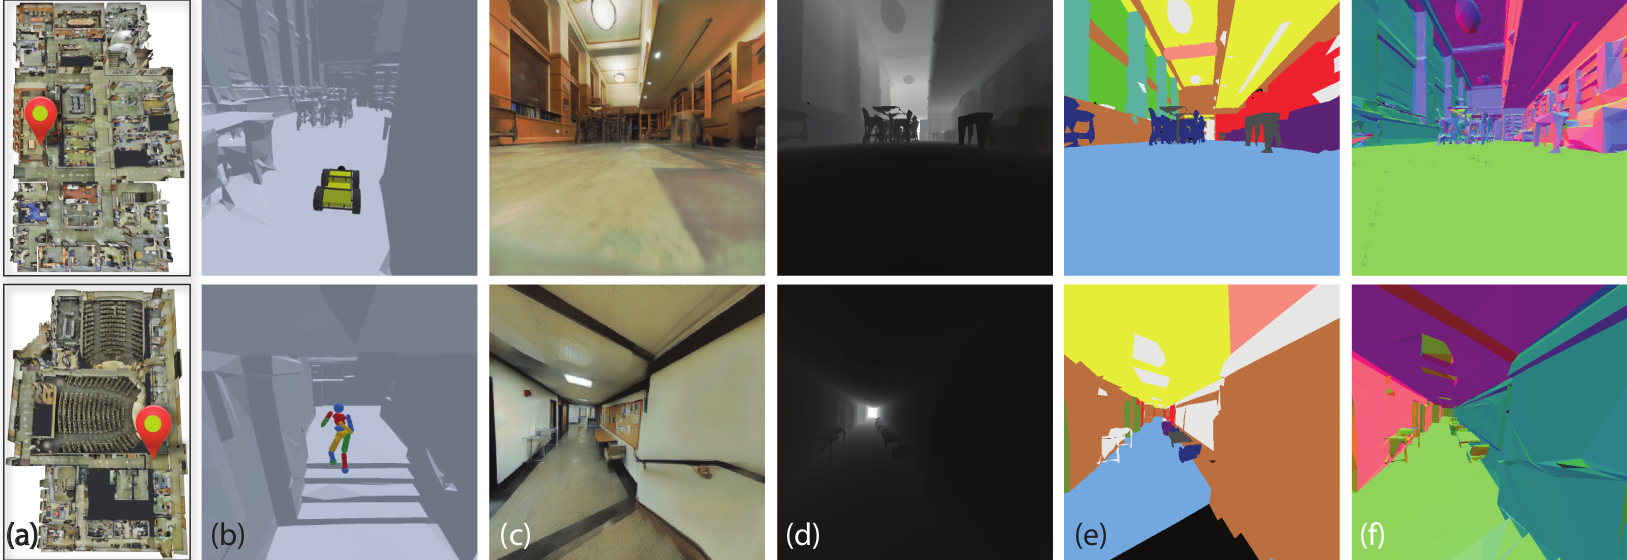
\includegraphics[width=0.99\linewidth]{images/gibson.png}
 	\caption{Two agents in Gibson Environment for real-world perception. The agent is active, embodied, and subject to constraints of physics and space
 		(a, b). It receives a constant stream of visual observations as if it had an on-board camera (c). It can also receive additional modalities, e.g. depth, semantic
 		labels, or normals (d, e, f). Image from \cite{gibson}.}
 \end{figure}
 
 Habitat is a platform for research in embodied artificial intelligence (AI) presented in \cite{habitat}. Habitat framework is composed by two modules: \textit{Habitat-Sim} and \textit{Habitat-API}. \textit{Habitat-Sim} is a flexible, high-performance 3D
 simulator with configurable agents, multiple sensors, and
 generic 3D dataset handling (with built-in support for Matterport3D \cite{matterport}, and Gibson \cite{gibson}). It is extremely fast when rendering a scene from Matterport3D, achieving thousand frames per second in a single thread and over 10,000 fps on a single GPU. \textit{Habitat-API} is a modular high-level library for end-to-end development of embodied AI algorithms concerning navigation, instruction following,
 and question answering.   
 
 In \cite{igibson}, \citeauthor{igibson} propose the Gibson Environment's evolution, called iGibson. This framework aims to unify several aspects of robot simulation, such as physics simulation for object interaction, high-quality simulated sensors data (RGB, depth, segmentation, LiDAR, and so on), integration with reinforcement learning frameworks, and realistic indoor scenes that reflect the objects' distribution of real indoor environments. This robotic simulator contains 15 fully interactive and visually realistic scenes with a total of 108 rooms. These scenes are generated  by annotating 3D reconstructions of real-world scans. The static meshes are then semantically annotated to obtain the ground truth segmentation of the various objects that populate a real scene. Then, these static environment models are converted into fully interactive scenes. This allows embodied active agents to engage in physical manipulation of articulated objects, changing the input sensor signals and the environment state. Furthermore, iGibson offers domain randomization procedures for materials (both visual appearances and dynamics properties) and object shapes applied to the object models in a scene. This facilitates the training of more robust end-to-end modules and improves their generalization properties in unseen scenes. In addition to the 15 interactive scenes, the authors support importing other datasets, such as CubiCasa5k \cite{cubicasa} and 3D-Front \cite{3dfront}. The first is a semi-automatically generated dataset of five thousand annotated floor plans of real-world homes in Finland, while the former is a large dataset of layouts designed by artists and interior designers. Both of them are converted from static scenes to fully interactive environments keeping their original structure. 
 

 